\vspace{-0.12in}

\subsection{Payload-Conditional Trajectory Generation}\label{sec:model}
\vspace{-0.1in}

We extend the diffusion policy architecture to condition trajectory generation on payload mass through global conditioning \cite{chi2023diffusionpolicy}. Unlike local conditioning where features influence each waypoint individually, global conditioning applies the mass embedding uniformly across the entire trajectory generation process, preserving dynamic feasibility across the generated motion (\Cref{fig:architecture}).
For each training trajectory $i$ with corresponding maximum supported payload mass $m_i \in \mathcal{D}$, we investigate four approaches to incorporate a target payload mass $p_i$ into an encoding vector $\mathcal{P}_i$.
The payload encoding $\mathcal{P}$ is concatenated with a diffusion timestep embedding to form a global conditioning vector, which is then integrated into $\epsilon_\theta$ through either additive or affine transform conditioning \cite{perez2018film}.% (\Cref{sec:misc-design}).
\begin{wrapfigure}{l}{0.48\textwidth}   % l or r = left / right, width = ~½ line
  \vspace{-1.6\baselineskip}            % tighten top gap (optional)
  \centering
  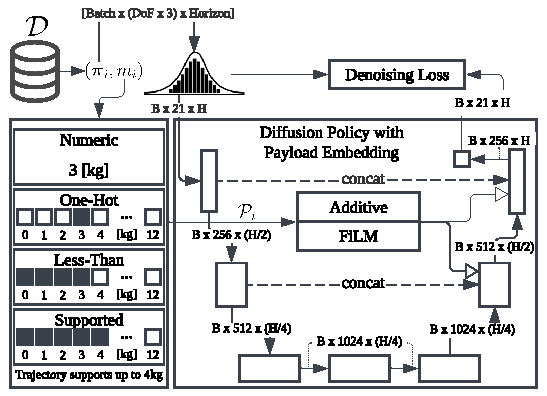
\includegraphics[width=\linewidth]{graphics/archnew.pdf}
  \caption{Our model conditions a 1D UNet denoising architecture \cite{chi2023diffusionpolicy} on various payload embeddings.}
  \label{fig:architecture}
  \vspace{-1.3\baselineskip}            % tighten bottom gap (optional)
\end{wrapfigure}
We consider the following approaches for designing $\mathcal{P}$.
\noindent\textbf{Numeric Input.} A random supported mass scalar $p_i \sim \mathcal{U}(0, m_i)$ is sampled and fed directly to the network. This approach naturally supports continuous payload values during inference, despite training on a discrete set of payload values.
\noindent\textbf{One-Hot Encoding.} For a system supporting payloads from $0-18$kg in $1$kg increments, a random supported mass $p_i \sim \mathcal{U}(0, m_i)$ is encoded as a $19$-dimensional binary vector with a single non-zero entry at index $\lceil p_i \rceil$.
While this categorical representation simplifies the learning task by discretizing the payload space, it constrains inference to the discrete payload values seen during training.
During inference, continuous payload masses must be quantized to their ceiling value $\lceil p \rceil$ before input to the denoising network, ensuring a tight upper bound for conservative operation.
\noindent\textbf{Less-Than Encoding.} This encoding exploits the logical constraint that trajectories supporting a given payload must also support all lighter payloads.
For a random supported mass $p_i \sim \mathcal{U}(0, m_i)$, we construct a $19$-dimensional binary vector where entries are $1$ for indices $j \leq \lceil p_i \rceil$ and $0$ otherwise.
This representation directly encodes the downward compatibility constraint into the input space, potentially improving the network's ability to learn and respect payload-dependent constraints.
During inference, continuous payload masses are similarly mapped to their ceiling value $\lceil p \rceil$ to construct the binary encoding.
\noindent\textbf{Supported-Range Encoding.}
This approach encodes the complete range of supported payloads for a given trajectory.
For training trajectory $i$ with maximum supported mass $m_i$, we construct a $19$-dimensional binary vector where entries are $1$ for indices $j \leq \lceil m_i \rceil$ and $0$ otherwise.
During training, this encoding preserves the full payload compatibility information from $\mathcal{D}$.
At inference time, for a target payload mass $p$, the encoding can be constructed either as a one-hot vector with a single non-zero entry at index $\lceil p \rceil$, or as a less-than encoding with ones for indices $j \leq \lceil p \rceil$.
This dual interpretation enables both trajectory generation for specific payloads and exploration of the learned manifold of payload-trajectory relationships.
Broadly, each encoding method presents trade-offs between generalization capability and training simplicity.